\documentclass[14pt, a4paper]{article}
\usepackage{minitoc}
\usepackage[left=3.00cm, right=2.5cm, top=2.00cm, bottom=2.00cm]{geometry}
\usepackage{amsmath}
\usepackage{amssymb}
\usepackage{amsthm}
\usepackage{mathtools}
\usepackage{graphicx}
%\usepackage{algpseudocode}
%\usepackage{algorithm}
\usepackage[ruled,vlined,linesnumbered]{algorithm2e}
\usepackage{blindtext}
\usepackage{setspace}
\usepackage[utf8]{inputenc}
\usepackage[utf8]{vietnam}
\usepackage[center]{caption}
\usepackage[shortlabels]{enumitem}
\usepackage{fancyhdr} % header, footer
\usepackage{hyperref} % loại bỏ border với mục lục và công thức
\usepackage[nonumberlist, nopostdot, nogroupskip]{glossaries}
\usepackage{glossary-superragged}
\usepackage{tikz,tkz-tab}
\usepackage{pythonhighlight}
\setglossarystyle{superraggedheaderborder}
\pagestyle{fancy}
%\usepackage[style=numeric,sortcites]{biblatex}
%\addbibresource{ref.bib}
%\usepackage[numbers]{natbib}
\usepackage{indentfirst}
\usepackage[natbib,backend=biber,style=ieee, sorting=ynt]{biblatex}
\bibliography{ref.bib}

\graphicspath{{./figures/}}

\fancyhf{}
%\rhead{\textbf{Môn học: Các phương pháp thống kê hiện đại trong nghiên cứu Xã hội học}}
\lhead{\textbf{GVHD: TS. Trịnh Quốc Anh}}
\rfoot{\thepage}
\lfoot{\textbf{Học viên thực hiện: Nguyễn Chí Thanh - 21007925}}
\renewcommand{\headrulewidth}{0.4pt}
\renewcommand{\footrulewidth}{0.4pt}
%
%\numberwithin{equation}{section}
%\numberwithin{algorithm}{section}
%\numberwithin{figure}{section}
%
%\setlength{\parindent}{0.5cm}
%
%\setcounter{secnumdepth}{3} % Cho phép subsubsection trong report
%\setcounter{tocdepth}{3} % Chèn subsubsection vào bảng mục lục

%\newtheorem{dl}{Định lý}
%\newtheorem{md}{Mệnh đề}
%\newtheorem{bd}{Bổ đề}
%\newtheorem{dn}{Định nghĩa}
%\newtheorem{hq}{Hệ quả}

%\newtheorem{baitap}{Bài tập}
%\newtheorem*{loigiai}{Lời giải}

%\numberwithin{dl}{section}
%\numberwithin{md}{section}
%\numberwithin{bd}{section}
%\numberwithin{dn}{section}
%\numberwithin{hq}{section}

\setlength{\parindent}{0cm}

\newtheorem{dl}{Định lý}
\newtheoremstyle{sltheorem}
{}                % Space above
{}                % Space below
{\normalfont}        % Theorem body font % (default is "\upshape")
{}                % Indent amount
{\bfseries}       % Theorem head font % (default is \mdseries)
{.}               % Punctuation after theorem head % default: no punctuation
{ }               % Space after theorem head
{}                % Theorem head spec
\theoremstyle{sltheorem}
\newtheorem{baitap}{Bài tập}
\newtheoremstyle{soltheorem}
{}                % Space above
{}                % Space below
{\normalfont}        % Theorem body font % (default is "\upshape")
{}                % Indent amount
{\bfseries}       % Theorem head font % (default is \mdseries)
{.}               % Punctuation after theorem head % default: no punctuation
{\newline}               % Space after theorem head
{}                % Theorem head spec
\theoremstyle{soltheorem}
\newtheorem*{loigiai}{Lời giải}

\onehalfspacing


\begin{document}
\begin{titlepage}

    \newcommand{\HRule}{\rule{\linewidth}{0.5mm}} % Defines a new command for the horizontal lines, change thickness here

    \center % Center everything on the page

    %----------------------------------------------------------------------------------------
    %	HEADING SECTIONS
    %----------------------------------------------------------------------------------------
    \textsc{\LARGE Đại học Quốc Gia Hà Nội}\\[0.5cm]
    \textsc{\LARGE Trường đại học Khoa học tự nhiên}\\[0.5cm] % Name of your university/college
    \textsc{\LARGE Khoa Toán - Cơ - Tin học}\\[0.5cm]

    
\includegraphics[scale=0.2]{HUS-logo.jpg}\\[0.5cm]

    \textsc{\Large Chuyên ngành: Khoa học dữ liệu}\\[0.5cm] % Major heading such as course name


    %----------------------------------------------------------------------------------------
    %	TITLE SECTION
    %----------------------------------------------------------------------------------------

    \HRule \\[0.4cm]
    { \huge \bfseries Bài tập môn học}\\[0.4cm] % Title of your document
    \HRule \\[1.5cm]

    \textsc{\Large Môn học: Các phương pháp thống kê hiện đại \\ trong nghiên cứu Xã hội học}\\[1cm] % Minor heading such as course title


    \textsc{\Large Bài tập 1}\\[1cm]


    %----------------------------------------------------------------------------------------
    %	AUTHOR SECTION
    %----------------------------------------------------------------------------------------
    \begin{minipage}{0.4\textwidth}
        \begin{flushleft} \large
        \emph{Giảng viên hướng dẫn:} \\
        TS. Trịnh Quốc Anh % Supervisor's Name
        \end{flushleft}
    \end{minipage}\\[0.5cm]

    \begin{minipage}{0.4\textwidth}
    \begin{flushleft} \large
    \emph{Học viên thực hiện:}\\
    Nguyễn Chí Thanh \\
    MSHV: 21007925 \\ % Your name
    Lớp: Khoa học dữ liệu - K4
    \end{flushleft}
    \end{minipage}


    % If you don't want a supervisor, uncomment the two lines below and remove the section above
    %\Large \emph{Author:}\\
    %John \textsc{Smith}\\[3cm] % Your name

    %----------------------------------------------------------------------------------------
    %	DATE SECTION
    %----------------------------------------------------------------------------------------

    % I don't want day because it is English
    % {\large \today}\\[2cm] % Date, change the \today to a set date if you want to be precise

    %----------------------------------------------------------------------------------------
    %	LOGO SECTION
    %----------------------------------------------------------------------------------------

    %\includegraphics{logo/rsz_3logo-khtn.png}\\[1cm] % Include a department/university logo - this will require the graphicx package

    %----------------------------------------------------------------------------------------

    \vfill % Fill the rest of the page with whitespace

\end{titlepage}

\nocite{*}

\newpage


\begin{baitap}
    Trả lời các câu hỏi 1 - 12, của quyển sách \cite{nolan2001stat}, trang 21 - 23
\end{baitap}

\begin{loigiai}
    Trả lời các câu hỏi 1 - 12, của quyển sách \cite{nolan2001stat}, trang 21 - 23
    \begin{enumerate}[wide, labelwidth=!, labelindent=0pt,label=\textbf{\arabic*}.]
        \item Sử dụng bảng \ref{tb:1.3} để ước lượng các phân vị phần tư của phân phối của số điếu thuốc đượt hút một ngày của các bà mẹ hút trong thời gian thai kỳ từ CHDS.

            \begin{table}[h!]
                \begin{center}
                    \begin{tabular}{|c|c|}
                        \hline
                        \textbf{Số điếu thuốc được hút} & \textbf{Tỷ lệ trong số người hút thuốc} \\  
                        \hline
                        0--5 & 16\% \\  
                        5--10 & 25\% \\  
                        10--15 & 14\% \\  
                        15--20 & 4\% \\  
                        20--30 & 32\% \\  
                        30--40 & 5\% \\  
                        40--60 & 4\% \\  
                        \hline
                        Tổng cộng & 100 \% \\
                        \hline
                    \end{tabular}
                \end{center}
                \caption{Bảng tần suất của số điếu thuốc được hút trong một ngày của 484 bà mẹ trong tập CHDS có hút thuốc trong thời gian thai kỳ,
                tỷ lệ phần trăm được làm tròn đến số nguyên gần nhất}
                \label{tb:1.3}
            \end{table}
        
        Ta có:
        \begin{equation*}
            \begin{aligned}
                &Q_1 = 5 + \dfrac{10 - 5}{25} \times (25 - 16) = 6.80 \\
                &Q_2 = 10 + \dfrac{15 - 10}{14} \times (50 - 41) = 13.21 \\
                &Q_3 = 20 + \dfrac{30 - 20}{32} \times (75 - 59) = 25
            \end{aligned}
        \end{equation*}

        \item Hợp bốn nhóm cuối trong bảng \ref{tb:1.3} thành một nhóm của phân phối số điếu thuốc đượt hút một ngày của các bà mẹ hút trong thời gian thai kỳ từ CHDS.
        Xây dựng histogram mới từ bảng thu được. Hình dạng thay đổi như nào so với histogram cũ?

        Ta có bảng phân phối mới sau khi hợp bốn nhóm cuối trong bảng \ref{tb:1.3}:

        \begin{table}[h!]
            \begin{center}
                \begin{tabular}{|c|c|}
                    \hline
                    \textbf{Số điếu thuốc được hút} & \textbf{Tỷ lệ trong số người hút thuốc} \\  
                    \hline
                    0--5 & 16\% \\  
                    5--10 & 25\% \\  
                    10--15 & 14\% \\  
                    15--60 & 45\% \\  
                    \hline
                    Tổng cộng & 100 \% \\
                    \hline
                \end{tabular}
            \end{center}
            \caption{Bản tần suất của số điếu thuốc được hút trong một ngày của 484 bà mẹ trong tập CHDS có hút thuốc trong thời gian thai kỳ,
            tỷ lệ phần trăm được làm tròn đến số nguyên gần nhất}
        \end{table}

        Ta sử dụng code để vẽ histogram mới:

        \begin{python}
import numpy as np
import matplotlib.pyplot as plt
            
            
lower = np.array([0, 5, 10, 15])
upper = np.array([5, 10, 15, 60])
            
percent = np.array([16, 25, 14, 45])
            
plt.bar(lower, percent/(upper-lower), width=upper - lower, ec="k", align="edge")
plt.xticks(lower.tolist() + [upper.tolist()[-1]], rotation=45)
plt.xlabel("Number of cigarettes (per day)")
plt.ylabel("Percent per cigarette")
plt.grid()
plt.show()
        \end{python}

        \begin{figure}[h!]
            \centering
            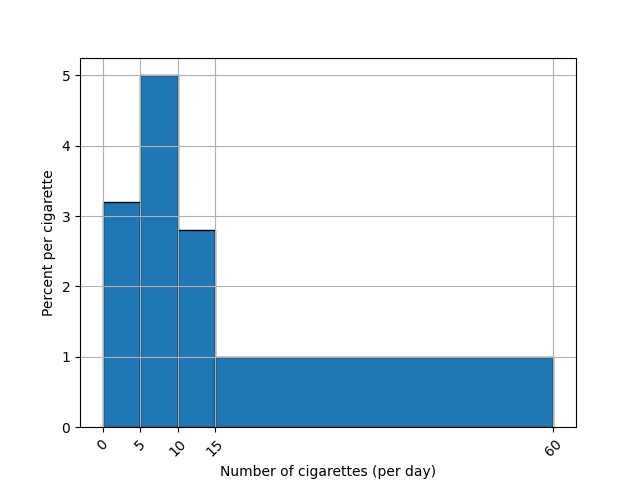
\includegraphics[scale=0.8]{2.png}
            \caption{histogram mới sau khi hợp bốn nhóm cuối bảng \ref{tb:1.3}}
        \end{figure}

        \item Ta xét histogram của tuổi của những người cha trong tập CHDS (hình \ref{fig:1.14}). Cột tương ứng với khoảng tuổi từ 35 đến 40 tuổi bị mất. Tìm chiều cao của cột này.
        \begin{figure}[h!]
            \centering
            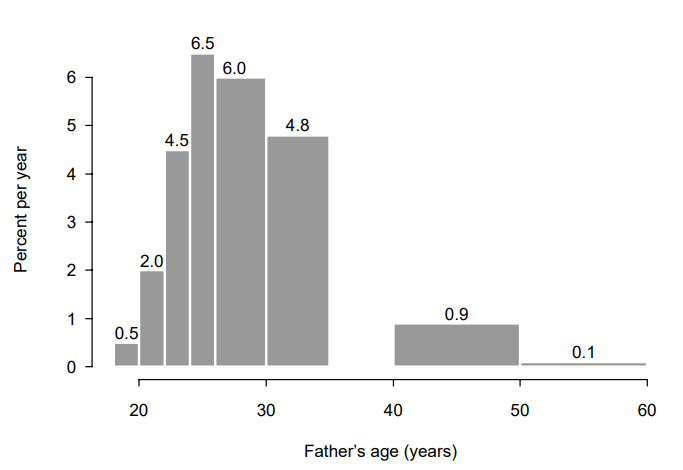
\includegraphics[scale=0.8]{1.14.png}
            \caption{Tuổi của những người cha (năm)}
            \label{fig:1.14}
        \end{figure}

        Ta đặt chiều cao của cột tương ứng với khoảng 35 - 40 tuổi là $x$:

        \begin{equation*}
            \begin{aligned}
                &0.5 \times 20 + 2.0 \times 2 + 4.5 \times 2 + 6.5 \times 2 + 6.0 \times 4 + 4.8 \times 5 + x \times 5 + 0.9 \times 10 + 0.1\times 10 = 100 \\
                &\Rightarrow x = \dfrac{100 - (0.5 \times 20 + 2.0 \times 2 + 4.5 \times 2 + 6.5 \times 2 + 6.0 \times 4 + 4.8 \times 5 + 0.9 \times 10 + 0.1\times 10)}{5} = \dfrac{100-94}{5}=1.2 \%
            \end{aligned}
        \end{equation*}

        Vậy chiều cao của cột tương ứng với khoảng 35 - 40 tuổi là 1.2 \%

        \item Ta xét quantile plot của chiều cao và cân nặng của những người cha trong CHDS (hình \ref{fig:1.15}). Hãy miêu tả hình dạng của các phân phối trên.
        \begin{figure}[h!]
            \centering
            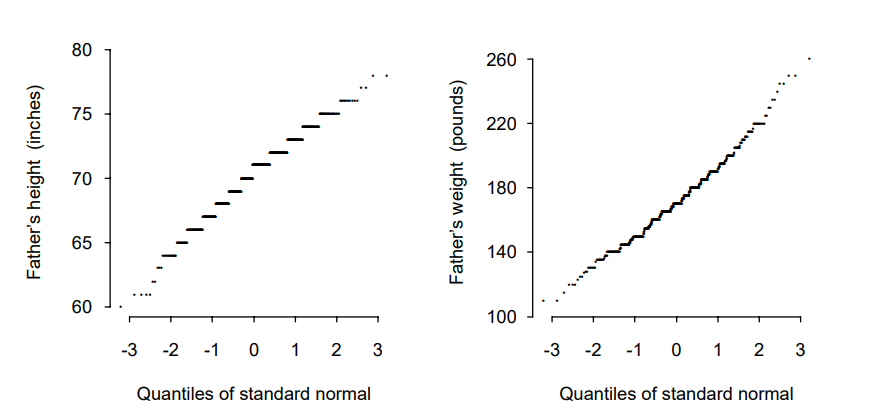
\includegraphics[scale=0.7]{1.15.png}
            \caption{Đồ thị quantile của chiều cao của những người cha (bên trái) và cân nặng (bên phải) trong tập CHDS.}
            \label{fig:1.15}
        \end{figure}

        Đồ thị quantile của chiều cao của những người cha cho thấy chiều cao được đo là một đại lượng rời rạc.
        Ta nhận thấy các điểm gần như nằm trên một đường thẳng cho thấy phân phối chiều cao của những người cha xấp xỉ phân phối chuẩn.
        
        \begin{figure}[h!]
            \centering
            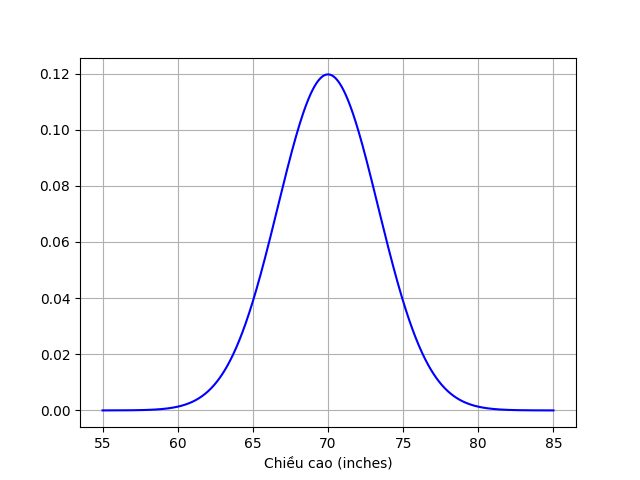
\includegraphics[scale=0.7]{4.1.png}
            \caption{Đồ thị hàm mật độ lý thuyết chiều cao của những người cha}
        \end{figure}

        Đồ thị quantile cân nặng của người cha cho thấy các điểm nằm khá sát trên một đường thẳng nên phân phối có dạng xấp xỉ phân phối chuẩn và phân phối khá đối xứng nhưng có khá ít điểm rơi vào khoảng biên và đa số các điểm tập trung ở khu vực trung nên cho ta thấy phân phối có hai bên đuôi khá nhẹ.
        
        \begin{figure}[h!]
            \centering
            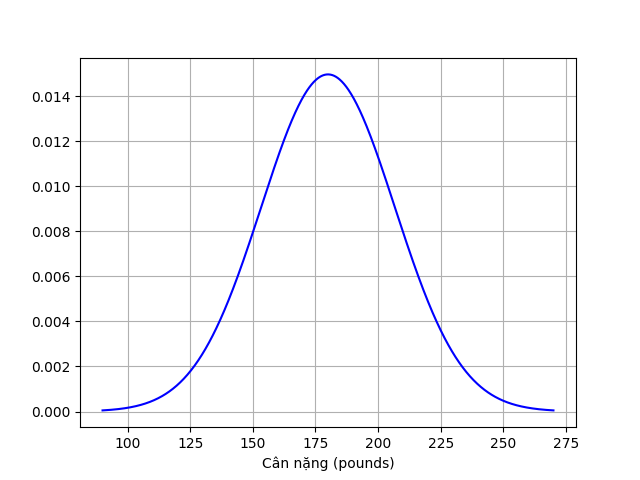
\includegraphics[scale=0.7]{4.2.png}
            \caption{Đồ thị hàm mật độ lý thuyết cân nặng của những người cha}
        \end{figure}

        \item Theo các phân vị 0.05, 0.1, \dots, 0.95 cho thời gian thai kỳ của em bé trong tập CHDS.
        Miêu tả hình dạng của phân phối của thời gian thai kỳ so với phân phối đều.
        252, 262, 267, 270, 272, 274, 276, 277, 278, 280, 281, 283, 284, 286, 288, 290, 292, 296, 302.
        
        Ta sử dụng đoạn code sau để vẽ đồ thị quantile của số liệu trên.

        \begin{python}
import numpy as np 
import pylab 
import scipy.stats as stats
import matplotlib.pyplot as plt
            
measurements = np.array([252, 262, 267, 270, 272, 274, 276, 277, 278, 280, 281, 283, 284, 286, 288, 290, 292, 296, 302])
quantiles = np.arange(1, measurements.shape[0] + 1) / (measurements.shape[0] + 1)
print(quantiles)
#plt.scatter(quantiles, measurements)
#plt.grid()
#plt.show()
stats.probplot(measurements, dist="uniform", plot=pylab)
pylab.title("Quantile plot")
pylab.xlabel("Quantiles of uniform")
pylab.ylabel("Gestational age")
pylab.grid()
pylab.show()
        \end{python}

        \begin{figure}[h!]
            \centering
            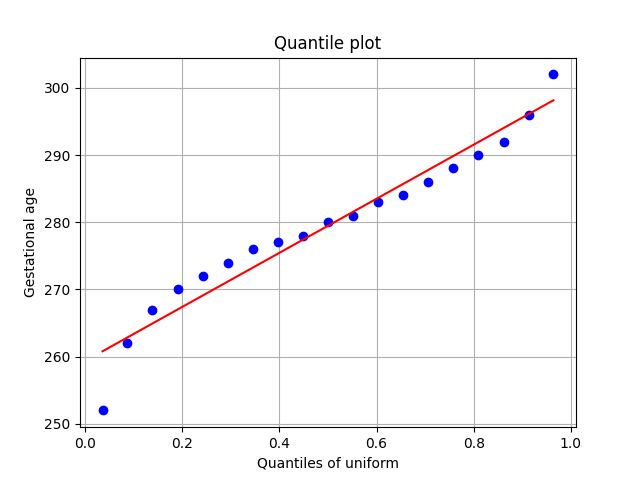
\includegraphics[scale=0.7]{5.png}
            \caption{Đồ thị quantile tương ứng với phân phối dữ liệu thời gian thai kỳ của em bé.}
        \end{figure}

        Từ đồ thị quantile ta nhận thấy phân phối thời gian thai kỳ của em bé có đuôi bên trái và bên phải dài hơn so với phân phối đều.

        \item Sử dụng xấp xỉ phân phối chuẩn ước lượng tỷ lệ của người mẹ trong tập CHDS có chiều cao từ 62 đến 64 inches đến nửa inch gần nhất (nằm giữa 61.5 và 64.5 inch).
        Chiều cao trung bình là 64 inch và độ lệch tiêu chuẩn SD là 2.5 inches.

        Ta gọi $X$ (inches) là chiều cao của các bà mẹ.
        \begin{equation*}
            X \sim \mathcal{N} (64; 2.5^2)
        \end{equation*}

        Ta cần tính $P(61.5 \leq X \leq 64.5)$:

        \begin{equation*}
            \begin{aligned}
                P (61.5 \leq X \leq 64.5) &= P \Big( \dfrac{61.5 - 64}{2.5} \leq \dfrac{Z - 64}{2.5} \leq \dfrac{64.5 - 64}{2.5} \Big) \\
                &= P (-1 \leq Z \leq 0.2) \\
                &= \Phi (0.2) - \Phi (-1) \\
                &= \Phi (0.2) - (1 - \Phi(1)) \\
                &= \Phi(0.2) + \Phi(1) - 1 \\
                &= 0.57926 + 0.84134 - 1 \\
                &= 0.4206
            \end{aligned}
        \end{equation*}

        \item Hai từ cần điền vào chỗ trống là:
        Vị trí thứ nhất: 2180
        Vị trí thứ hai: 2.64

        \item Ta giả sử có 100 quan sát từ phân phối chuẩn tắc.
        Tỷ lệ trong số các quan sát này mà ta kỳ vọng nằm ngoài whisker của một đồ thị whisker and box?


        Đối với phân phối chuẩn tắc ta có $z_{0.25}=-0.6745$ và $z_{0.75}=0.6745$ hay $Q_1=-0.6745$ và $Q_3=0.6745$.
        Vậy $IQR=Q_3 - Q_1 = 0.6745 - (-0.6745)=1.349$.

        Xác suất để một quan sát nằm ngoài whisker là:

        \begin{equation*}
            \begin{aligned}
                P (Z < Q_1 - 1.5 \times IQR \cup Z > Q_3 + 1.5 \times IQR) &= P (Z < Q_1 - 1.5 \times IQR) + P (Z > Q_3 + 1.5 \times IQR) \\
                &= P(Z < -0.6745 - 1.5 \times 1.349) + P (Z > 0.6745 + 1.5 \times 1.349) \\
                &= P(Z < -2.648) + P (Z > 2.698) \\
                &= \Phi(-2.698) + (1 - \Phi(2.698)) \\
                &= (1 - \Phi(2.698)) + (1 - \Phi(2.698)) \\
                &= 2 \times (1 - \Phi(2.698)) \\
                &= 0.00698 = 0.698 \%
            \end{aligned}
        \end{equation*}

        Như vậy tỷ lệ số quan sát nằm ngoài whisker của một đồ thị whisker and box là 0.698 \%.
        Và như vậy chỉ có khoảng 1 quan sát nằm ngoài whisker của một đồ thị whisker and box.

        \item Tạo một bảng của tình trạng hôn nhân cho biết tỷ lệ người hút thuốc và không hút thuốc trong từng nhóm tình trạng hôn nhân của các bà mẹ trong nghiên cứu Missouri (hình \ref{fig:Table1.16}).
        \begin{figure}[h!]
            \centering
            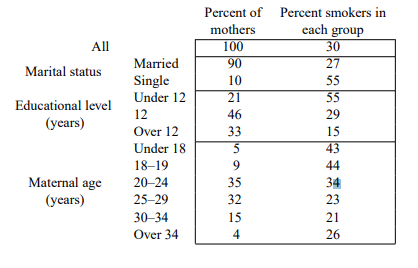
\includegraphics[scale=0.8]{Table1.6.png}
            \caption{Tỷ lệ người mẹ hút thuốc theo từng nhóm đặc trưng theo tình trạng hôn nhân, học vấn và tuổi}
            \label{fig:Table1.16}
        \end{figure}

        \begin{table}[h!]
            \begin{center}
                \begin{tabular}{|c|c|c|}
                    \hline
                    Tình trạng hôn nhân& Tỷ lệ người hút thuốc & Tỷ lệ người không hút thuốc \\  
                    \hline
                    Đã kết hôn & 27 \% & 73 \% \\
                    \hline
                    Độc thân & 55 \% & 45 \% \\
                    \hline
                \end{tabular}
            \end{center}
            \caption{Tỷ lệ các bà mẹ hút thuốc trong thời kỳ mang thai theo tình trạng hôn nhân trong nghiên cứu Missouri}
            \label{tb:Marital-status}
        \end{table}
        Bảng của tình trạng hôn nhân cho biết tỷ lệ người hút thuốc và không hút thuốc trong từng nhóm tình trạng hôn nhân của các bà mẹ trong nghiên cứu Missouri được thể hiện ở bảng \ref{tb:Marital-status}

        \item Tạo một biểu đồ cột chồng thể hiện tỷ lệ về các cấp độ học vấn cho cả các bà mẹ hút thuốc và không hút thuốc trong thời gian thai kỳ trong nghiên cứu Missouri (hình \ref{fig:Table1.16})
        
        Ta gọi $A$ là sự kiện một bà mẹ ở nhóm trình độ dưới lớp 12.
        Ta gọi $B$ là sự kiện một bà mẹ ở nhóm trình độ lớp 12.
        Ta gọi $C$ là sự kiện một bà mẹ ở nhóm trình độ trên lớp 12.

        Ta gọi $Y$ là sự kiện một bà mẹ hút thuốc trong thời gian thai kỳ.

        Ta cần tính $P(A \vert Y), P(B \vert Y), P(C \vert Y)$ và $P(A \vert \overline{Y}), P(B \vert \overline{Y}), P(C \vert \overline{Y})$.

        Ta có $P(A)=0.21, P(B)=0.46, P(C)=0.33, P(Y \vert A)=0.55, P(Y \vert B)=0.29, P(Y \vert C)=0.15$

        Ta xét hệ đầy đủ $A, B, C$, theo công thức xác suất đầy đủ:

        \begin{equation*}
            \begin{aligned}
                P(Y) &= P(A) P (Y \vert A) + P(B) P (Y \vert B) + P(C) P(Y \vert C) \\
                &= 0.21 \times 0.55 + 0.46 \times 0.29 + 0.33 \times 0.15 \\
                &= 0.2984 \\
                \Rightarrow P(\overline{Y}) &= 1 - P(Y) = 1 - 0.2984 = 0.7016
            \end{aligned}
        \end{equation*}

        \begin{equation*}
            \begin{aligned}
                P(A \vert Y) &= \dfrac{P(AY)}{P(Y)}=\dfrac{P(A)P(Y\vert A)}{P(Y)}=\dfrac{0.21\times 0.55}{0.2984}=0.3871 \\
                P(B \vert Y) &= \dfrac{P(BY)}{P(Y)}=\dfrac{P(B)P(Y\vert B)}{P(Y)}=\dfrac{0.46\times 0.29}{0.2984}=0.4471 \\
                P(C \vert Y) &= \dfrac{P(CY)}{P(Y)}=\dfrac{P(C)P(Y\vert C)}{P(Y)}=\dfrac{0.33\times 0.15}{0.2984}=0.1658 \\
                P(A \vert \overline{Y}) &= \dfrac{P(A\overline{Y})}{P(\overline{Y})}=\dfrac{P(A)P(\overline{Y}\vert A)}{P(\overline{Y})}=\dfrac{0.21\times 0.45}{0.7016}=0.1347 \\
                P(B \vert \overline{Y}) &= \dfrac{P(B\overline{Y})}{P(\overline{Y})}=\dfrac{P(B)P(\overline{Y}\vert B)}{P(\overline{Y})}=\dfrac{0.46\times 0.71}{0.7016}=0.4655 \\
                P(C \vert \overline{Y}) &= \dfrac{P(C\overline{Y})}{P(\overline{Y})}=\dfrac{P(C)P(\overline{Y}\vert C)}{P(\overline{Y})}=\dfrac{0.33\times 0.85}{0.7016}=0.3998 \\
            \end{aligned}
        \end{equation*}

        Ta thực hiện code vẽ hiện biểu đồ cột chồng thể hiện tỷ lệ về các cấp độ học vấn cho cả các bà mẹ hút thuốc và không hút thuốc trong thời gian thai kỳ trong nghiên cứu Missouri:

        \begin{python}
import pandas as pd
import numpy as np
import matplotlib.pyplot as plt
            
df = pd.DataFrame({"Under 12": [0.3871, 0.1347],
                    "12": [0.4471, 0.4655],
                    "Over 12": [0.1658, 0.3998]},
                    index=["Smoked", "Non Smoked"])
            
ax = df.plot(kind="bar", stacked=True, color=["red", "yellow", "blue"])
            
for rect in ax.patches:
    # Find where everything is located
    height = rect.get_height()
    width = rect.get_width()
    x = rect.get_x()
    y = rect.get_y()
                
    # The height of the bar is the data value and can be used as the label
    label_text = f'{height:.4f}'  # f'{height:.2f}' to format decimal values
                
    # ax.text(x, y, text)
    label_x = x + width / 2
    label_y = y + height / 2
            
    # plot only when height is greater than specified value
    if height > 0:
        ax.text(label_x, label_y, label_text, ha='center', va='center', fontsize=8)
            
plt.xlabel("Smoking status")
plt.xticks(rotation=0)
plt.ylabel("Percent in each group")

plt.title("Percentage of each education level for both smokers and nonsmokers")

plt.show()
        \end{python}
        \begin{figure}[h!]
            \centering
            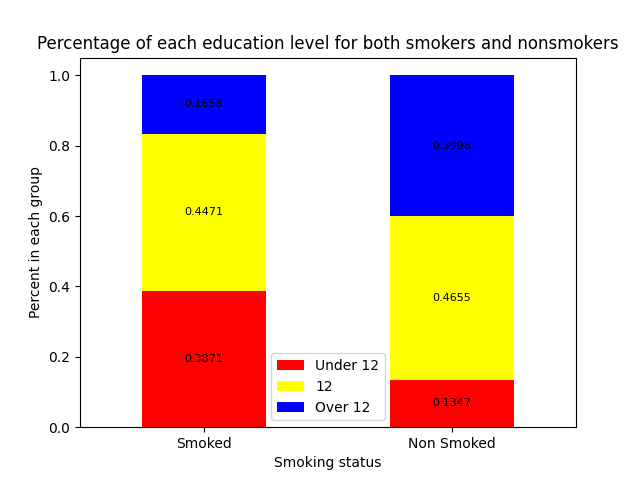
\includegraphics[scale=0.8]{10.png}
            \caption{Biểu đồ cột chồng thể hiện tỷ lệ về các cấp độ học vấn cho cả các bà mẹ hút thuốc và không hút thuốc trong thời gian thai kỳ trong nghiên cứu Missouri}
        \end{figure}

        \item Tạo một biểu đồ cột theo tuổi và tình trạng hút thuốc trong thời gian thai kỳ của các bà mẹ trong nghiên cứu Missouri (hình \ref{fig:Table1.16}).
        Trong từng nhóm, cột thể hiện tỷ lệ các bà mẹ hút thuốc trong nhóm.

        Ta thực hiện code vẽ biểu đồ cột thể hiện tỷ lệ các bà mẹ hút thuốc trong từng nhóm tuổi:

        \begin{python}
import numpy as np
import matplotlib.pyplot as plt

data = {"Under 18": 43, "18-19": 44, "20-24": 34, "25-29": 23, "30-34": 21, "Over 34": 26}

x = list(data.keys())
y = list(data.values())

fig, ax = plt.subplots(figsize=(9, 9))
ax.bar(x, y, color ="blue", width = 0.4)
plt.bar_label(ax.containers[0], label_type='edge', color='red', rotation=90, fontsize=15, padding=10)
 
plt.xlabel("Age group")
plt.ylabel("Percentage of mothers who smokes")
plt.title("Bar graph of age and smoking status")
plt.grid()
plt.show()
        \end{python}

        \begin{figure}[h!]
            \centering
            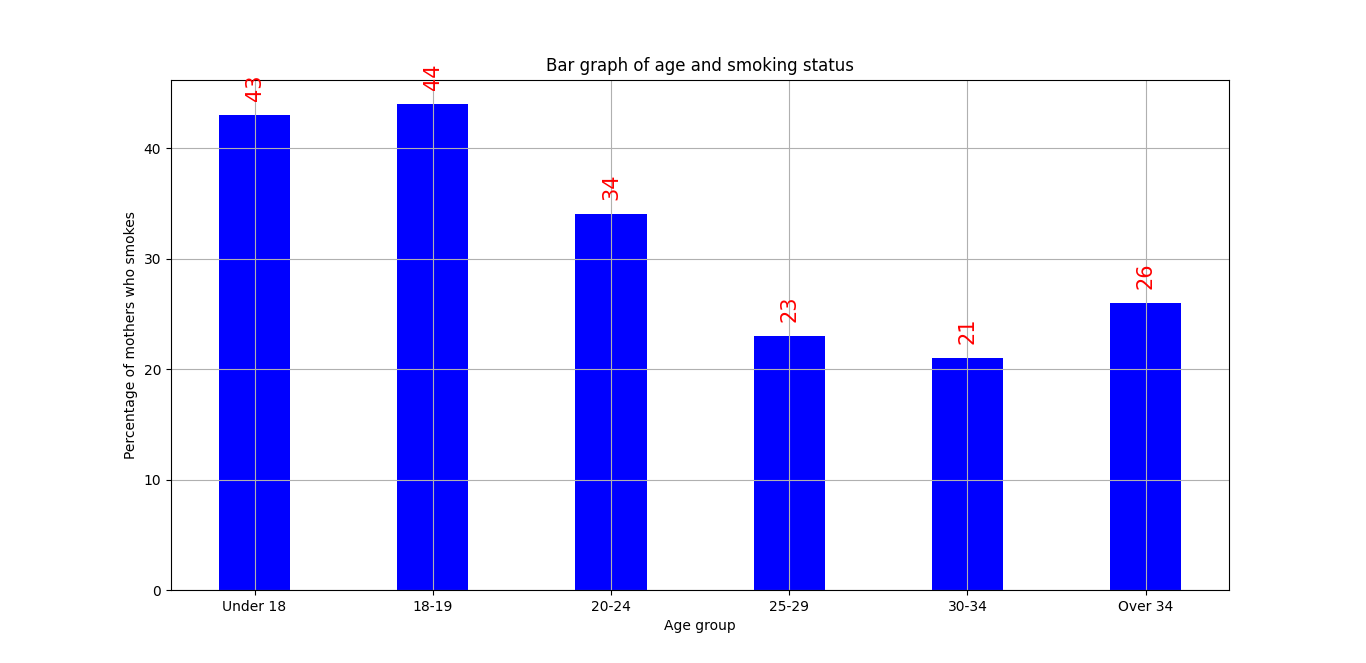
\includegraphics[scale=0.4]{11.png}
            \caption{Biểu đồ cột theo tuổi và tình trạng hút thuốc trong thời gian thai kỳ của các bà mẹ trong nghiên cứu Missouri}
        \end{figure}

        Ta tính độ tương quan giữa độ tuổi và tỷ lệ hút thuốc

        \item Trong nghiên cứu Missouri, cân nặng trung bình khi sinh của các em bé mà có mẹ hút thuốc trong thời gian thai kỳ là 3180 grams và độ lệch chuẩn SD 500 grams.
        Cân nặng trung bình và độ lệch chuẩn SD trong đơn vị ounces. Biết rằng 0.0035 ounces tương đương 1 gram.

        Ta có cân nặng trung bình trong đơn vị ounces là: $3180\times 0.035=111.3$ (ounces) và độ lệch chuẩn SD trong đơn vị ounces là: $500 \times 0.035=17.5$ (ounces).

        \textbf{19.} Chứng minh rằng trung bình $\bar{x}$ là hằng số cực tiểu hóa hàm sai lệch bình phương tương ứng với $c$:

        \begin{equation*}
            \sum_{i=1}^n (x_i - c)^2
        \end{equation*}

        Ta đặt $f(c) = \sum_{i=1}^n (x_i - c)^2$. Ta biến đổi:

        \begin{equation*}
            \begin{aligned}
                f(c) &= \sum_{i=1}^n (x_i - c)^2 \\
                &= \sum_{i=1}^n (x_i^2 - 2x_i c + c^2) \\
                &= \sum_{i=1}^n x_i^2 - 2(\sum_{i=1}^n x_i)c + n c^2 \\
                &= n\Bigg(c - \dfrac{\sum_{i=1}^n x_i}{n}\Bigg)^2 + \Bigg(\sum_{i=1}^n x_i^2 - \dfrac{(\sum_{i=1}^n x_i)^2}{n}\Bigg)
            \end{aligned}
        \end{equation*}

        Ta nhận thấy thành phần $\Bigg(\sum_{i=1}^n x_i^2 - \dfrac{(\sum_{i=1}^n x_i)^2}{n}\Bigg)$ không phụ thuộc vào $c$ vì vậy $f(c)$ nhỏ nhất khi $\Bigg(c - \dfrac{\sum_{i=1}^n x_i}{n}\Bigg)^2=0$ hay $c= \dfrac{\sum_{i=1}^n x_i}{n} = \bar{x}$ (điều phải chứng minh).

        \textbf{20.} Chứng minh rằng trung vị $\tilde{x}$ của $x_1, \dots, x_n$ là hằng số cực tiểu hóa sai lệch tuyệt đối tương ứng với $c$:

        \begin{equation*}
            \sum_{i=1}^n \lvert x_i - c \vert
        \end{equation*}

        Ta đặt $f(c) = \sum_{i=1}^n \lvert x_i - c \vert$
        Ta giả sử dãy $x_1, \dots, x_n$ được sắp xếp theo chiều không giảm hay $x_1 \leq x_2 \leq \dots \leq x_n$.
        Ta chọn một số $c$ sao cho $c < x_1$, khi đó:

        \begin{equation*}
            f(c) = \sum_{i=1}^n \lvert x_i - c \vert = \sum_{i=1}^n (x_i - c)
        \end{equation*}

        Nếu $c$ tăng dần nhưng vẫn nhỏ hơn $x_1$ thì từng thành phần $x_i - c$ sẽ giảm đến khi $c$ đạt đến $x_1$,
        vì vậy $f(x_1) < f(x) \thickspace \forall c < x_1$.
        Ta chọn một số $c$ sao cho $x_k \leq c \leq c + d \leq x_{k+1}(d > 0)$, khi đó:

        \begin{equation*}
            \begin{aligned}
                f(c + d) &= \sum_{i=1}^k (c + d - x_i) + \sum_{i=k+1}^n (x_i - (c + d)) \\
                &= dk + \sum_{i=1}^k (c - x_i) - d(n-k) + \sum_{i=k+1}^n (x_i - c) \\
                &= d(2k -n) + \sum_{i=1}^k (c - x_i) + \sum_{i=k+1}^n (x_i - c) \\
                &= d(2k - n) + f(c) \\
            \Rightarrow f(c + d) - f(c) &= d(2k - n)
            \end{aligned}
        \end{equation*}
        Ta nhận thấy khi $2k < n$, thì $f(c + d) < f(c)$, $2k = n$ thì $f(c+d)=f(c)$, $2k > n$ thì $f(c+d) > f(c)$.
        Hay khi $k$ tăng dần trước khi đạt đến $n/2$ thì f(c) giảm, và khi $k$ lớn hơn $n / 2$ thì f(c) tăng, nghĩa là f(c) sẽ đạt cực tiểu tại $k=n/2$ nghĩa là $k=n/2$ ở chính giữa dãy số đã được sắp xếp theo thứ tự không giảm.
        Vì vậy $f(c) = \sum_{i=1}^n \lvert x_i - c \vert = \sum_{i=1}^n (x_i - c)$ đạt cực tiểu khi $c$ chính là trung vị của dãy $x_1, \dots, x_n$ (điều phải chứng minh).
    \end{enumerate}
\end{loigiai}

\newpage
\printbibliography[title={TÀI LIỆU THAM KHẢO}]

\end{document}